\section{Zusätzliche Kommunikation}
\label{Kommuniaktion}
In den bisherigen Betrachtungen der Varianten zum \textit{cheating-husbands}-Rätsel war der Informationsaustausch zwischen den Ehefrauen stark eingeschränkt.
Die Kommunikation einer Ehefrau war darauf beschränkt mitzuteilen, ob sie weiß, dass sie betrogen wurde.
Wenn sie dies mit Sicherheit sagen konnte, erschießt sie ihren Ehemann in der Nacht, die anderen Ehefrauen hörten den Schuss und wussten somit, dass eine andere Ehefrau sich sicher war, dass ihr Ehemann betrogen hat.\\
Wenn diese Beschränkung aufgehoben wird, können ohne die Mächtigkeit des Systems zu erhöhen, wesentlich effizientere Kommunikationsprotokolle genutzt werden, um das Problem zu lösen.
Um dies zu zeigen abstrahieren wir nun wieder von dem, als sehr entscheidend festgestellten, Nachrichtensystem. 
Nachrichten der Königin werden daher ohne Verzögerung verteilt, und jeder Ehefrau ist dies bekannt.
Bei der ursprünglichen Lösung aus der Motivation wurde das Problem in n Tagen Tagen gelöst, wobei n die Anzahl der untreuen Ehemänner ist.
Y. Moses et al. \cite{moses1986cheating} (vgl. S.175) zeigen, dass das Problem mit zusätzlicher Kommunikation mit einem Algorithmus gelöst werden kann, der höchstens drei Tage benötigt.
Die Mächtigkeit des Systems bleibt hier insofern gleich, als das weiterhin nur über Schüsse um Mitternacht kommuniziert werden kann. Dies entspricht einer binären Nachricht pro Nacht, entweder sind ein oder mehr Schüsse in der Nacht gefallen oder keiner.\\
Zunächst können wir mit einer an \cite{moses1986cheating} angelegten Überlegung beweisen, dass es kein Protokoll gibt, das weniger als drei Nächte unabhängig von der Probleminstanz benötigt:\\

Betrachten wir eine Probleminstanz mit k untreuen Ehemännern.
Im Allgemeinen kann es nun zwei verschiedene Anzahlen von untreuen Ehemännern geben, von denen die Ehefrauen wissen.
Entweder kennen sie alle k, wenn sie selbst nicht betrogen wurden, oder sie kennen $k-1$, wenn sie betrogen wurden.
Da keine der Ehefrauen weiß, ob sie betrogen wurde, wissen sie nur, dass die wahre Anzahl untreuer Ehemänner entweder $k_i$ oder $k_i+1$ ist.
Somit gibt es Ehefrauen die wissen, dass es $k-1$ oder $k$ und welche die wissen, dass es $k$ oder $k+1$ untreue Ehemänner gibt.
Wenn die wahre Anzahl untreuer Ehemänner bekannt ist, ist das System vollständig bestimmt, jede Ehefrau weiß dann, ob sie ihren Mann erschießen muss.
Jede Nacht kann allerdings nur eine binäre Information bekannt gemacht werden, daher kann im Allgemeinen jede Nacht nur einer der drei möglichen Anzahlen von untreuen Ehemännern ausgeschlossen werden.

So könnte ein Schuss in der ersten Nacht bedeuten, dass es entweder $x$ oder $y$ untreue Ehemänner sind. Eine zweite Nacht müsste dann noch abgewartet werden, um eindeutig zu bestimmen, welcher der beiden Fälle der Wahrheit entspricht. Wenn kein Schuss in der ersten Nacht fallen würde, wäre hier klar, dass es weder $x$ noch $y$ untreue Ehemänner sind. Es kann also durchaus Fälle geben, in denen das Problem in zwei Nächten gelöst ist. Es kann aber kein Protokoll geben, dass das Problem unabhängig von $k$ immer in weniger als drei Nächten löst.\\

\subsection{Protokoll mit zusätzlicher Kommunikation}

Die folgende leicht modifizierte Version des Kommunikationsprotokolls von Y. Moses et al. \cite{moses1986cheating} (vgl. S.175) ist eine optimale Lösung für das \textit{cheating husbands}-Rätsel mit zusätzlicher Kommunikation, in dem Sinne, dass es maximal drei Tage benötigt, um jegliche Probleminstanz korrekt zu lösen:
\begin{itemize}
	\item 1. Falls eine Ehefrau von $k_0$ (mit $k_0 \text{ mod } 3 = 0$) weiß, schießt sie in der ersten Nacht in die Luft.
	\item 2. Falls eine Ehefrau von $k_1$ (mit $k_1 \text{ mod } 3 = 1$) weiß und in der ersten Nacht kein Schuss gefallen ist, erschießt sie ihren Ehemann in der zweiten Nacht.
	\item 3. Falls eine Ehefrau von $k_2$ (mit $k_2 \text{ mod } 3 = 2$) weiß und in der ersten Nacht ein Schuss gefallen ist, erschießt sie ihren Ehemann in der zweiten Nacht.
	\item 4. Falls in den ersten beiden Nächten kein Schuss gefallen ist, erschießen alle Ehefrauen ihren Mann in der dritten Nacht.
	\item 5. Falls in der ersten Nacht ein Schuss gefallen ist und in der zweiten nicht, erschießen alle Ehefrauen, die in der ersten Nacht bereits geschossen haben, ihren Mann in der dritten Nacht. 
\end{itemize}
Das Protokoll kann folgendermaßen erklärt werden:\\
Zu 2.: Hier wurde $k_0$ ausgeschlossen. Es gibt zwei Fälle, in denen niemand von $k_0$ einige hingegen von $k_1$ untreuen Ehemännern wissen: Manche Ehefrauen kennen $k_1$ und andere $k_2$ untreue Ehemänner oder alle Ehefrauen wissen von $k_1$ betrogenen Ehefrauen. Aufgrund der Modulo-Eigenschaft kann entweder $k_1 = k_0-2$ und $k_2 = k_0-1$ oder $k_1 = k_0+1$ und $k_2 = k_0+2$ sein. Entweder sind also alle Frauen betrogen worden, oder es gibt welche, die von einem untreuen Ehemann mehr als $k_1$ wissen. Die Ehefrauen, für die der zweite Fall des Protokolls zutrifft, müssen also betrogen worden sein.\\
Zu 3.: Hier wurde $k_1$ ausgeschlossen,  gleiche Argumentation wie zu 2.\\
Zu 4.: Sowohl $k_0$, als auch $k_1$ sind ausgeschlossen worden, jede Ehefrau weiß von $k_2$ untreuen Ehemännern, also sind alle Ehefrauen betrogen worden.\\
Zu 5.: Gleiche Argumentation, wie bei 2. und 3., nur dass hier $k_2$ ausgeschlossen wurde. \\
Es sind somit alle möglichen Fälle abgedeckt: Die Ehefrauen wissen von $k_i-1$ und $k_i$, von $k_i$ und $k_i+1$, nur von $k-1$, nur von $k$ oder nur von $k+1$ untreuen Ehemännern. Alle Regeln sind korrekt und somit auch das gesamte Kommunikationsprotokoll.\\

Die Fähigkeit untereinander zu Kommunizieren ermöglicht es, dass in diesem Kommunikationsprotokoll keine Notwendigkeit darin besteht, dass die Königin verkündet, dass es mindestens einen untreuen Ehemann gibt. Tatsächlich funktioniert das Protokoll auch für den Fall, dass es keinen untreuen Ehemann gibt.
Mit Hilfe der Veranschaulichung von Kripke-Modellen können wir nun die korrekte Funktionsweise des Protokolls an dem Beispiel aus Kapitel \ref{Kripke-Modelle} betrachten:\\
Von der ersten zur zweiten Nacht wird der in Abbildung \ref{kom_(0,1,1)} dargestellte Übergang vollzogen, dass Problem wird also direkt gelöst.
Der korrekte Zustand ist (0,1,1), somit ist die tatsächliche Anzahl der untreuen Ehemänner $k=2$. Die Ehefrauen 2 und 3 kennen $k_1 = 1$ untreue Ehemänner und Ehefrau 1 kennt $k_2 = 2$ untreue Ehemänner. Es gibt also keine Ehefrau, die $k_0$ untreue Ehemänner kennt, sodass in der ersten Nacht kein Schuss gefallen ist. Dementsprechend sind in Abbildung \ref{kom_(0,1,1)} die Zustände (0,0,0) und (1,1,1) ausgeschlossen worden.
Die Zustände (1,0,0), (0,1,0) und (0,0,1) sind ebenso weggefallen, da es in ihnen eine Frau hätten geben müssen, die von keinem (also von $k_0$) untreuen Ehemann weiß. Alle Ehefrauen wissen also nach einer Nacht, dass sie sich in Zustand (0,1,1) befinden.

\begin{figure}
	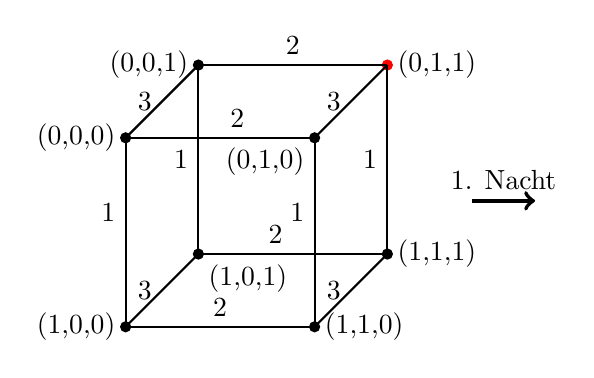
\begin{tikzpicture}[thick,scale=0.2]
	\coordinate[label={180:\text{(1,0,0)}}] (UVL) at (0,0,12);
	\coordinate[label={0:\text{(1,1,0)}}] (UVR) at (12,0,12);
	\coordinate[label={180:\text{(0,0,0)}}] (OVL) at (0,12,12);
	\coordinate[label={-120:\text{(0,1,0)}}] (OVR) at (12,12,12);
	\coordinate[label={-86:\text{(1,0,1)}}] (UHL) at (0,0,0);
	\coordinate[label={0:\text{(1,1,1)}}] (UHR) at (12,0,0);
	\coordinate[label={180:\text{(0,0,1)}}] (OHL) at (0,12,0);
	\coordinate[label={0:\text{(0,1,1)}}] (OHR) at (12,12,0);
	
	\draw[fill=black] (UVL) circle (8pt);
	\draw[fill=black] (UVR) circle (8pt);
	\draw[fill=black] (OVL) circle (8pt);
	\draw[fill=black] (OVR) circle (8pt);
	\draw[fill=black] (UHL) circle (8pt);
	\draw[fill=black] (UHR) circle (8pt);
	\draw[fill=black] (OHL) circle (8pt);
	\filldraw[color=red] (OHR) circle (8pt);
	
	\draw (UVL) -- node[above] {2} (UVR);
	\draw (UVL) -- node[above left] {1} (OVL);
	\draw (UVL) -- node[left] {3} (UHL);
	\draw (OVR) -- node[above right] {2} (OVL);
	\draw (OVR) -- node[left] {3} (OHR);
	\draw (OVR) -- node[above left] {1} (UVR);
	\draw (OHL) -- node[left] {3} (OVL);
	\draw (OHL) -- node[above] {2} (OHR);
	\draw (OHL) -- node[left] {1} (UHL);
	\draw (UHR) -- node[left] {3} (UVR);
	\draw (UHR) -- node[left] {1} (OHR);
	\draw (UHR) -- node[above left] {2} (UHL);	
	
	\draw[line width=1.5pt,->] (22,8,12) -- node[above] {1. Nacht} (26,8,12); 	
	\end{tikzpicture}
	\qquad
	\hspace*{-0.7cm}
	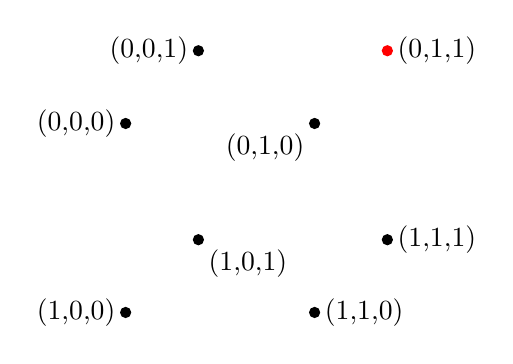
\begin{tikzpicture}[thick,scale=0.2]
	\coordinate[label={180:\text{(1,0,0)}}] (UVL) at (0,0,12);
	\coordinate[label={0:\text{(1,1,0)}}] (UVR) at (12,0,12);
	\coordinate[label={180:\text{(0,0,0)}}] (OVL) at (0,12,12);
	\coordinate[label={-120:\text{(0,1,0)}}] (OVR) at (12,12,12);
	\coordinate[label={-86:\text{(1,0,1)}}] (UHL) at (0,0,0);
	\coordinate[label={0:\text{(1,1,1)}}] (UHR) at (12,0,0);
	\coordinate[label={180:\text{(0,0,1)}}] (OHL) at (0,12,0);
	\coordinate[label={0:\text{(0,1,1)}}] (OHR) at (12,12,0);
	
	\draw[fill=black] (UVL) circle (8pt);
	\draw[fill=black] (UVR) circle (8pt);
	\draw[fill=black] (OVL) circle (8pt);
	\draw[fill=black] (OVR) circle (8pt);
	\draw[fill=black] (UHL) circle (8pt);
	\draw[fill=black] (UHR) circle (8pt);
	\draw[fill=black] (OHL) circle (8pt);
	\filldraw[color=red] (OHR) circle (8pt);		
	\end{tikzpicture}
	\caption{Übergang vom ersten zum zweiten Tag im \textit{cheating husbands}-Rätsels mit zusätzlicher Kommunikation ausgehend vom Zustand (0,1,1).}
	\label{kom_(0,1,1)}
\end{figure}

Betrachten wir den Fall, dass (0,0,0) der wahre Zustand ist. Alle Ehefrauen kennen also $k_0 = 0$ untreue Ehemänner.
In der ersten Nacht sind also Schüsse zu hören, da niemand drei untreue Ehemänner kennen kann, wird Zustand (1,1,1) ausgeschlossen, die Zustände mit zwei untreuen Ehemännern können dann auch ausgeschlossen werden, da es entweder keinen oder einen untreuen Ehemann geben muss.

\begin{figure}
	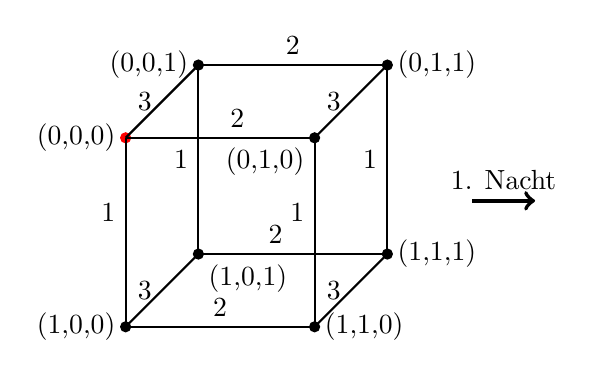
\begin{tikzpicture}[thick,scale=0.2]
	\coordinate[label={180:\text{(1,0,0)}}] (UVL) at (0,0,12);
	\coordinate[label={0:\text{(1,1,0)}}] (UVR) at (12,0,12);
	\coordinate[label={180:\text{(0,0,0)}}] (OVL) at (0,12,12);
	\coordinate[label={-120:\text{(0,1,0)}}] (OVR) at (12,12,12);
	\coordinate[label={-86:\text{(1,0,1)}}] (UHL) at (0,0,0);
	\coordinate[label={0:\text{(1,1,1)}}] (UHR) at (12,0,0);
	\coordinate[label={180:\text{(0,0,1)}}] (OHL) at (0,12,0);
	\coordinate[label={0:\text{(0,1,1)}}] (OHR) at (12,12,0);
	
	\draw[fill=black] (UVL) circle (8pt);
	\draw[fill=black] (UVR) circle (8pt);
	\filldraw[color=red] (OVL) circle (8pt);
	\draw[fill=black] (OVR) circle (8pt);
	\draw[fill=black] (UHL) circle (8pt);
	\draw[fill=black] (UHR) circle (8pt);
	\draw[fill=black] (OHL) circle (8pt);
	\filldraw[color=black] (OHR) circle (8pt);
	
	\draw (UVL) -- node[above] {2} (UVR);
	\draw (UVL) -- node[above left] {1} (OVL);
	\draw (UVL) -- node[left] {3} (UHL);
	\draw (OVR) -- node[above right] {2} (OVL);
	\draw (OVR) -- node[left] {3} (OHR);
	\draw (OVR) -- node[above left] {1} (UVR);
	\draw (OHL) -- node[left] {3} (OVL);
	\draw (OHL) -- node[above] {2} (OHR);
	\draw (OHL) -- node[left] {1} (UHL);
	\draw (UHR) -- node[left] {3} (UVR);
	\draw (UHR) -- node[left] {1} (OHR);
	\draw (UHR) -- node[above left] {2} (UHL);	
	
	\draw[line width=1.5pt,->] (22,8,12) -- node[above] {1. Nacht} (26,8,12); 	
	\end{tikzpicture}
	\qquad
	\hspace*{-0.7cm}
	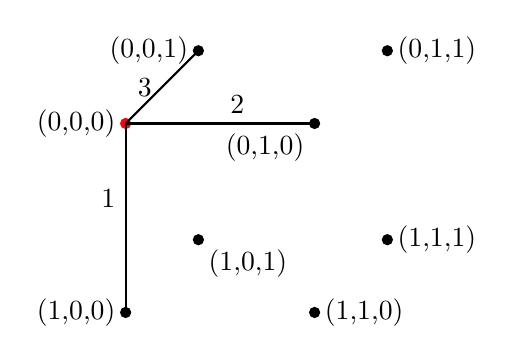
\begin{tikzpicture}[thick,scale=0.2]
	\coordinate[label={180:\text{(1,0,0)}}] (UVL) at (0,0,12);
	\coordinate[label={0:\text{(1,1,0)}}] (UVR) at (12,0,12);
	\coordinate[label={180:\text{(0,0,0)}}] (OVL) at (0,12,12);
	\coordinate[label={-120:\text{(0,1,0)}}] (OVR) at (12,12,12);
	\coordinate[label={-86:\text{(1,0,1)}}] (UHL) at (0,0,0);
	\coordinate[label={0:\text{(1,1,1)}}] (UHR) at (12,0,0);
	\coordinate[label={180:\text{(0,0,1)}}] (OHL) at (0,12,0);
	\coordinate[label={0:\text{(0,1,1)}}] (OHR) at (12,12,0);
	
	\draw[fill=black] (UVL) circle (8pt);
	\draw[fill=black] (UVR) circle (8pt);
	\filldraw[color=red] (OVL) circle (8pt);
	\draw[fill=black] (OVR) circle (8pt);
	\draw[fill=black] (UHL) circle (8pt);
	\draw[fill=black] (UHR) circle (8pt);
	\draw[fill=black] (OHL) circle (8pt);
	\filldraw[color=black] (OHR) circle (8pt);
	
	\draw (UVL) -- node[above left] {1} (OVL);
	\draw (OVR) -- node[above right] {2} (OVL);
	\draw (OHL) -- node[left] {3} (OVL);		
	\end{tikzpicture}
	\caption{Übergang vom ersten zum zweiten Tag im \textit{cheating husbands}-Rätsels mit zusätzlicher Kommunikation}
	\label{kom_(0,0,0)}
\end{figure}